\documentclass[
  bibliography=totoc,     % Literatur im Inhaltsverzeichnis
  captions=tableheading,  % Tabellenüberschriften
  titlepage=firstiscover, % Titelseite ist Deckblatt
]{scrartcl}

% Paket float verbessern
\usepackage{scrhack}

% Warnung, falls nochmal kompiliert werden muss
\usepackage[aux]{rerunfilecheck}

% unverzichtbare Mathe-Befehle
\usepackage{amsmath}
% viele Mathe-Symbole
\usepackage{amssymb}
% Erweiterungen für amsmath
\usepackage{mathtools}

% Fonteinstellungen
\usepackage{fontspec}
% Latin Modern Fonts werden automatisch geladen
% Alternativ zum Beispiel:
%\setromanfont{Libertinus Serif}
%\setsansfont{Libertinus Sans}
%\setmonofont{Libertinus Mono}

% Wenn man andere Schriftarten gesetzt hat,
% sollte man das Seiten-Layout neu berechnen lassen
\recalctypearea{}

% deutsche Spracheinstellungen
\usepackage[main=ngerman]{babel}


\usepackage[
  math-style=ISO,    % ┐
  bold-style=ISO,    % │
  sans-style=italic, % │ ISO-Standard folgen
  nabla=upright,     % │
  partial=upright,   % ┘
  warnings-off={           % ┐
    mathtools-colon,       % │ unnötige Warnungen ausschalten
    mathtools-overbracket, % │
  },                       % ┘
]{unicode-math}

% traditionelle Fonts für Mathematik
\setmathfont{Latin Modern Math}
% Alternativ zum Beispiel:
%\setmathfont{Libertinus Math}

\setmathfont{XITS Math}[range={scr, bfscr}]
\setmathfont{XITS Math}[range={cal, bfcal}, StylisticSet=1]

% Zahlen und Einheiten
\usepackage[
  locale=DE,                   % deutsche Einstellungen
  separate-uncertainty=true,   % immer Fehler mit \pm
  per-mode=symbol-or-fraction, % / in inline math, fraction in display math
]{siunitx}

% chemische Formeln
\usepackage[
  version=4,
  math-greek=default, % ┐ mit unicode-math zusammenarbeiten
  text-greek=default, % ┘
]{mhchem}

% richtige Anführungszeichen
\usepackage[autostyle]{csquotes}

% schöne Brüche im Text
\usepackage{xfrac}

% Standardplatzierung für Floats einstellen
\usepackage{float}
\floatplacement{figure}{htbp}
\floatplacement{table}{htbp}

% Floats innerhalb einer Section halten
\usepackage[
  section, % Floats innerhalb der Section halten
  below,   % unterhalb der Section aber auf der selben Seite ist ok
]{placeins}

% Seite drehen für breite Tabellen: landscape Umgebung
\usepackage{pdflscape}

% Captions schöner machen.
\usepackage[
  labelfont=bf,        % Tabelle x: Abbildung y: ist jetzt fett
  font=small,          % Schrift etwas kleiner als Dokument
  width=0.9\textwidth, % maximale Breite einer Caption schmaler
]{caption}
% subfigure, subtable, subref
\usepackage{subcaption}


% Grafiken können eingebunden werden
\usepackage{graphicx}
% größere Variation von Dateinamen möglich
%\usepackage{grffile}

% schöne Tabellen
\usepackage{booktabs}

% Verbesserungen am Schriftbild
\usepackage{microtype}
\setlength{\parindent}{0pt}

% Literaturverzeichnis
\usepackage[
  backend=biber,
]{biblatex}
% Quellendatenbank
\addbibresource{lit.bib}
\addbibresource{programme.bib}

% Hyperlinks im Dokument
\usepackage[
  german,
  unicode,        % Unicode in PDF-Attributen erlauben
  pdfusetitle,    % Titel, Autoren und Datum als PDF-Attribute
  pdfcreator={},  % ┐ PDF-Attribute säubern
  pdfproducer={}, % ┘
]{hyperref}
% erweiterte Bookmarks im PDF
\usepackage{bookmark}

% Trennung von Wörtern mit Strichen
\usepackage[shortcuts]{extdash}

% Import PDFs
\usepackage{pdfpages}


\usepackage{graphicx}






\title{
  Wiederholungsaufgaben\\
  \small{\emph{Experimentelle Übung II, SoSe 2020}}
  }
\author{%
  Marcel Kebekus\\%
  \href{mailto:marcel.kebekus@tu-dortmund.de}{\small{marcel.kebekus@tu-dortmund.de}}%
}
\date{%
  \small{Abgabetermin: 27.04.2020} 
}
\makeatletter         
\def\@maketitle{
\raggedright
\includegraphics[width=\textwidth]{bilder/lo_TU-Do 2008/logo_rgb_jpg}\\[8ex]
\begin{center}
{\Huge \bfseries \sffamily \@title }\\[4ex] 
{\Large  \@author}\\[4ex] 
\@date\\[8ex]
\publishers\\
\end{center}}
%\makeatother


\begin{document}
\maketitle
%\thispagestyle{empty}
%\tableofcontents
\newpage
\section{Aufgabe 1 - Bedeutung der Begriffe}
\subsection{Mittelwert}
    Der Mittelwert $\mu$ eines Datensatzes, ist dessen im durchschnitt angenommener Wert.

    \begin{equation*}
        \mu=\frac{1}{n}\sum_{i=0}^n x_i
    \end{equation*}
\subsection{Standardabweichung}
    Die Standartabweichung $\sigma$ gibt an, wie weit jeder Wert eines Datensatzes im durchschnitt von 
    dem Mittelwert abweicht.\\
    Sie beschreibt somit eine Diffuson der Messwerte, um den Mittelwert. Je größer der Wert, desto
    größer ist die Streuung der Werte um den Mittelwert.
    \begin{equation*}
        \sigma = \sqrt{\frac{\sum_{i=0}^n(x_i-\mu)^2}{n}}
    \end{equation*}
\subsection{Unterscheidung zwischen Streuung der Messwerte und der Fehler des Mittelwerts}
    Mit Streuung der Messwerte ist hiermit die Standardabweichung gemeint, also der Fehler der Einzelmessung.
    Der (mittlere) Fehler des Mittelwertes $\Delta \mu$ unterschiedet sich dabei um den Faktor $1/\sqrt{n}$ von diesem, sodass
    \begin{equation*}
        \Delta \mu = \frac{\sigma}{\sqrt{n}}.
    \end{equation*}

\newpage
\section{Aufgabe 2 - Volumenberechnung}
    Berechnen des Volumens eines Holzylinders mit dem Außenradius $R_a$, Innenradius $R_i$ und
    der Höhe $h$:
    \begin{align*}
        R_{a}=(15 \pm 1) \si{cm},\\
        R_{i}=(10 \pm 1) \si{cm},\\
        h=(20 \pm 1) \si{cm}.\\
    \end{align*}
    Da die Größen fehlerbehaftet sind, erfolgt die allgmeiner Fehlerfortpflanzung nach Gauß
    \begin{equation*}
        \Delta f(x_i)=\sqrt{\sum_{i=0}^n \left(\frac{df}{dx_i}\cdot \Delta x_i \right) ^2},
    \end{equation*}
    und spezifisch für den Holzylinder mit
    \begin{align*}
        \Delta V &= \sqrt{\left(\frac{dV}{dR_{a}}\cdot \Delta R_{a}\right)^2 + \left(\frac{dV}{dR_{i}}\cdot \Delta R_{i}\right)^2 + \left(\frac{dV}{dh}\cdot \Delta h\right)^2},\\\\
        \Delta V &= \sqrt{(2 \pi h R_a \Delta R_a)^2 + (-2 \pi h R_i \Delta R_i)^2 + (\pi (R_a^2-R_i^2) \cdot \Delta h)^2} .
    \end{align*}
    Mit dem Volumen $V$ eines Holzylinders
    \begin{equation*}
        V= \pi h \cdot(R_{a}^2-R_{i}^2),
    \end{equation*}
    ergibt sich schließlich das Gesamtvolumen $V_{ges}$
    \begin{equation*}
        V_{ges}=(2500\pi \pm 732\pi)\; \si{cm^3}.
    \end{equation*}
\newpage
\section{Lineare Regression}
    In einem Versuchteil wurden die folgenden Daten für Liniennummer $N_{Linie}$
    und Spannung $U$ aufgenommen.
    Die Liniennummern $N_{Linie}$ sollen dabei gemäß der Formel in Abstände $D$ umgerechnet werden 
    \begin{equation}
        D=(N_{Linie}-1) \cdot 6 \si{mm.}
        \label{eqn:formel}
    \end{equation}

    \begin{table}[H]
        \centering
        \begin{tabular}{c c c}
            \toprule
            Liniennummer $N_{Linie}$ & $U\;/\;$V & $D\;/\;$mm \\
            \midrule
            1&-19.5&0\\
            2&-16.1&6\\
            3&-12.4&12\\
            4&-9.6&18\\
            5&-6.2&24\\
            6&-2.4&30\\
            7&1.2&36\\
            8&5.1&42\\
            9&8.3&48\\
            \bottomrule
        \end{tabular}
        \caption{Messdaten Liniennummer $N_{Linie}$ und Spannung $U$ mit berechneten
            Abständen $D$ nach Gl. \ref{eqn:formel}}
        \label{tab:tabelle}
    \end{table}

    Trägt man nun die Spannung $U$ gegen den Abstand $D$ auf,so folgt für eine lineare 
    Regression nach 
    \begin{equation}
        U=m\cdot D + n,
        \label{eqn:gerade}
    \end{equation}
    für die Steigung $m$ und den y-Achsenabschnitt $n$
    \begin{align*}
        m&=(0.581\pm0.007) \si{\volt\per\mm}\\
        n&=(-19.68\pm0.19) \si{V}\\.
    \end{align*}
    \begin{figure}[H]
        \centering
        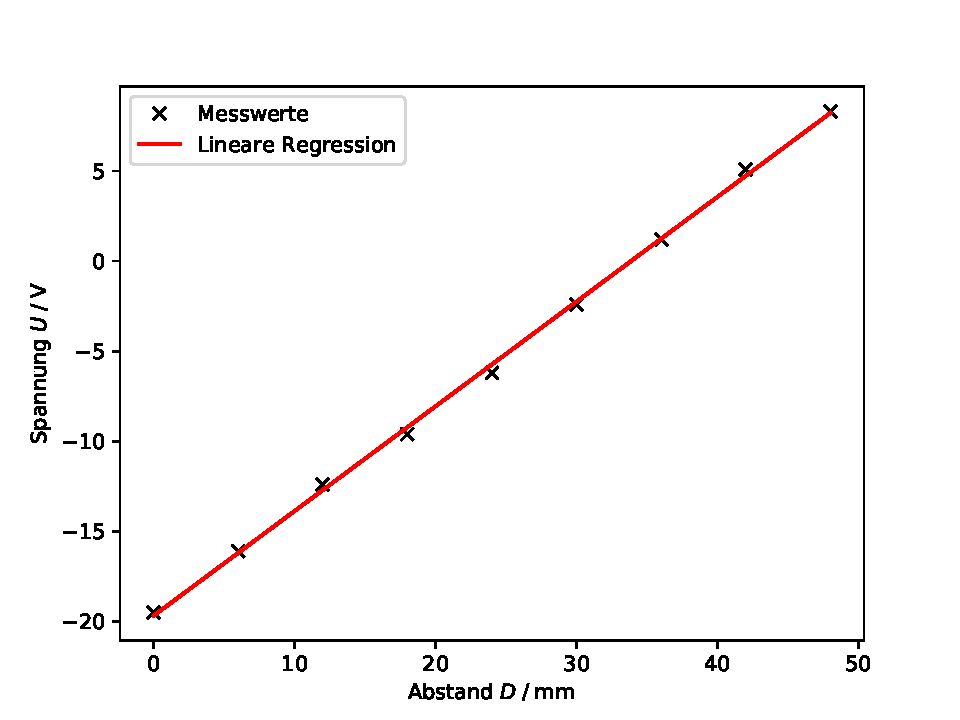
\includegraphics[width=0.8\textwidth]{plot.pdf}
        \caption{In der Grapik wird die Spannung $U$ gegen den Abstand $D$ aufgetragen, sowie 
        die lineare Regression nach der Geradengleichung \ref{eqn:gerade} und derer Parameter.}
    \end{figure}
%\nocite{*}
%\printbibliography


\end{document}
